% !TEX root=../../report.tex

\section{SOLL-Workflow \enquote{Event planen}}
\label{workflow}

Die Hauptfunktion des EventManagers soll die Eventplanung sein. Aus diesem Grund ist es besonders wichtig, diesen Arbeitsablauf genau zu planen und zu optimieren.

\begin{figure}[ht]
\centering
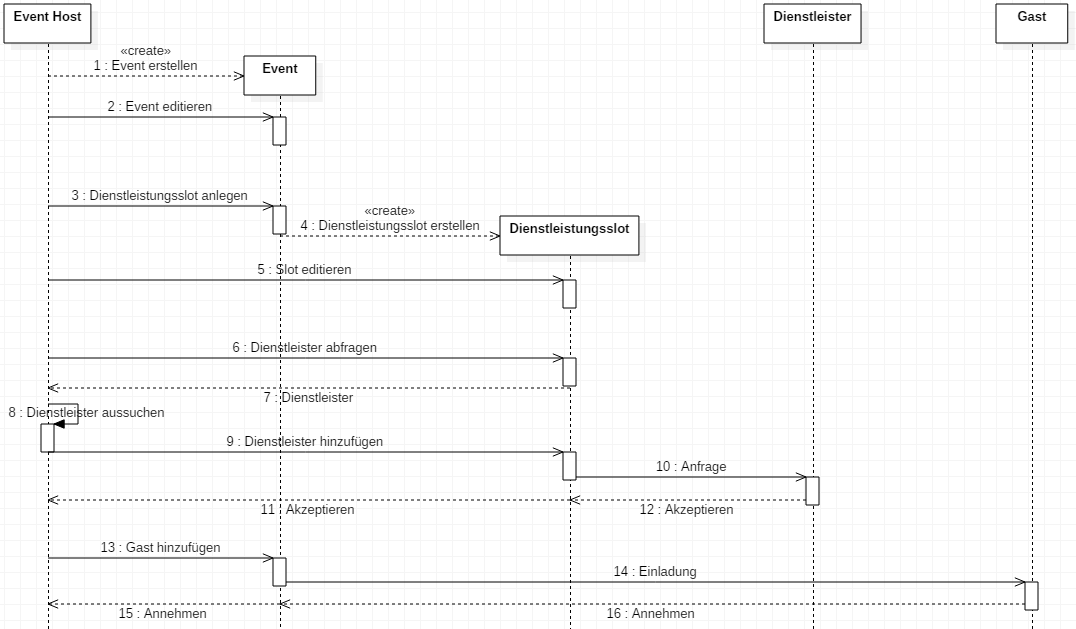
\includegraphics[width=\textwidth]{res/images/WorkflowCreateEvent.png}
\caption{Sequenzdiagramm Event planen}
\label{wf1}
\end{figure}

In Teamarbeit wird dieser Workflow ausgearbeitet und in einem \gls{uml} Sequenzdiagramm festgehalten, welches in \myautoref{wf1} zu sehen ist. Die erste Aufgabe, die von einem Veranstalter ausgeführt werden muss, ist die Erstellung des eigentlichen Events. Hierbei müssen bereits einige Daten erfasst werden, die das Team für essentiell erachtet. Dazu gehören der Titel und die Start- und Endzeit. Optional können die restlichen Felder gefüllt werden, zu denen die Beschreibung, das vorgesehene Budget, sowie der Veranstaltungsort gehören. Diese Daten sollen während des gesamten Planungsvorgangs weiterhin geändert werden können. Ist das Event angelegt, so kann sich um die Dienstleistungen gekümmert werden. Dazu können für jede vorgesehene Dienstleistung entsprechende Slots angelegt werden. Hierbei muss die Dienstleistungskategorie angegeben werden, wie zum Beispiel Musiker, Caterer, oder Hallenvermieter. Des Weiteren wird auch hier die Start- und Endzeit benötigt. Optional kann ein Budget angegeben werden, das man für diese Dienstleistung ausgeben möchte. Auch der Dienstleistungsslot soll während des gesamten Planungsvorgangs änderbar bleiben. Pro Slot kann der Veranstalter jetzt einen Dienstleister suchen. Die Auswahl wird automatisch auf die Kategorie eingeschränkt. Durch das Hinzufügen stellt das System automatisch eine Anfrage an den entsprechenden Dienstleister. Jetzt kann diese vom Dienstleister akzeptiert werden. Damit wird er dem Slot zugeordnet.

Als letztes fehlen noch die Gäste der Veranstaltung. Diese werden vom Veranstalter eingeladen, indem er sie über die Benutzerkonten sucht und schließlich einlädt. Die Zu- und Absagen werden dem Veranstalter im Event angezeigt, sodass er die Übersicht behält, welche und wieviele Gäste am Event teilnehmen werden.
